\documentclass[10pt,a4paper]{article}
\usepackage[margin=25mm]{geometry}
\usepackage{amsmath,amssymb,booktabs,array,graphicx}
\usepackage[T1]{fontenc}
\usepackage{lmodern}
\usepackage[hidelinks]{hyperref}
\usepackage{microtype}
\setlength{\parskip}{4pt}
\setlength{\parindent}{1em}
\setlength{\emergencystretch}{2em}
\renewcommand{\arraystretch}{1.13}
\newcommand{\HawkingT}{T_{\mathrm H}}
\newcommand{\cphase}{c_{\mathrm{phase}}}
\newcommand{\cefh}{c_{\mathrm{EFH}}}
\newcommand{\cext}{c_{\mathrm{ext}}}
\newcommand{\bext}{b_{0,\mathrm{ext}}}
\newcommand{\bcand}{b_{0,\mathrm{loc}}}
\newcommand{\dd}{\mathrm d}
\newcommand{\Ai}{\mathrm{Ai}}
\newcommand{\Bi}{\mathrm{Bi}}
\title{Finite-dispersion temperature corrections in stationary\newline
quartic-superluminal Hawking scattering}
\author{Tatsuhiko Takimoto\\\small Independent researcher}
\date{Version 1.2, 22 October 2026}
\begin{document}
\maketitle
\begin{abstract}
We examine the frequency dependence of a temperature defined by the ratio
of Bogoliubov coefficients for a stationary, one-dimensional flow with
quartic superluminal dispersion. Two independently developed numerical
methods, stabilized spatial integration and a global Chebyshev boundary-value
method, give compatible scattering data within the recorded comparison
precision. For 19 smooth profiles, the stored extrapolations of the
$\omega^2/\Lambda^2$ coefficient agree with a local derivative expression
to an absolute difference below $1.3\times10^{-3}$. This expression is a
short consequence of the Leonhardt--Robertson phase-integral formula;
the numerical comparison concerns its applicability to the full four-mode
wave equation. The results differ from the coefficient obtained by directly
applying Eq.~(133) of Del Porro, Liberati and Schneider. The domains and
orders of approximation must be reconciled before interpreting that
difference as a disagreement of equivalent predictions. For the
low-frequency temperature offset we apply the zero-frequency matching
procedure of Coutant and Weinfurtner to this wave equation. Under stated
regularity, regularization and matching assumptions, the $\omega\to0$ limit
of the ratio temperature reduces, without approximation in the dispersion
scale $\Lambda$, to a Wronskian and two integrals of one solution of a
second-order equation. A formal expansion about the horizon turning point
then gives the relative offset $\kappa\,g'''(0)/(12\Lambda^2)$, where $g$
expresses $v'$ as a function of $1+v$. This is a formal asymptotic
calculation: global matching and a remainder bound are not proved. It is
supported numerically: the zero-frequency reduction agrees with
extrapolated $\omega\to0$ scattering limits within $1.3\times10^{-10}$ in
$28$ cases, and predictions recorded before any zero-frequency or
scattering calculation for two new profile families agree with the offsets
extrapolated from those limits within $1.1\times10^{-7}$. A separately
written scattering code reproduces the predicted offset for four profiles,
two of them new, within $1.1\times10^{-7}$.
\end{abstract}

\section{Question and relation to previous work}
\label{sec:intro}
The leading Hawking temperature is robust in many dispersive models; for
example, Corley and Jacobson analysed horizon mode conversion with
high-frequency dispersion \cite{CJ}, and Unruh and Sch\"utzhold examined
the conditions under which the effect is universal \cite{US}.
Finite-dispersion deviations, in turn, contain information about the background
flow and the observable used to define a temperature. We ask which
coefficient is measured by full stationary scattering when the low-frequency
offset and the frequency curvature are separated. With sound speed set to
one, the horizon is at $v(0)=-1$, its slope is $\kappa=v'(0)>0$, and
$\HawkingT=\kappa/(2\pi)$; $\hbar=k_B=1$ throughout.

The analysis builds on distinct contributions. Macher and Parentani
developed the three-channel scattering description and separated an
effective low-frequency temperature from spectral curvature
\cite{MP}. Coutant, Parentani and Finazzi developed analytical connection
and momentum-space methods \cite{CPF}. Leonhardt and Robertson expressed
the temperature through an inverse-flow phase integral \cite{LR}.
Moreno-Ruiz and Bermudez applied such methods to nonlinear profiles and
compared analytical and numerical temperatures \cite{MRB}.
Himemoto and Tanaka studied finite-dispersion corrections involving
higher background derivatives \cite{HT}. Del Porro, Liberati and
Schneider developed a tunneling method for analogue Hawking quanta, for
flows with and without horizons and with sub- or superluminal dispersion
\cite{DPLS25}, and then connected the tunneling and Bogoliubov
descriptions through an effective horizon \cite{DPLS}. Eq.~(133) of the
latter work supplies the comparison coefficient in this report. Coutant and Weinfurtner showed how to read
low-frequency scattering coefficients from a zero-frequency solution of a
second-order equation and its first-order frequency correction
\cite{CWKdV,CWBdG}; our low-frequency calculation follows that procedure.

The numerical quantities of interest are the coefficients in
\begin{equation}
 \frac{T(\omega,\Lambda)}{\HawkingT}-1
 \simeq \frac{b_0\kappa^2+c\omega^2}{\Lambda^2}+\cdots .
 \label{eq:target}
\end{equation}
Here $\simeq$ specifies an asymptotic interpretation of finite-range fits,
rather than a uniform error theorem. We distinguish the formal
phase-integral value of $c$, the measured full-scattering coefficients,
and the low-frequency coefficient $b_0$, which Section~\ref{sec:b0}
obtains by a formal asymptotic calculation. The calculation is a comparison
of these quantities, rather than a claim that dispersive temperature
corrections, the phase-integral method or the zero-frequency method are
new.

\section{Wave equation, channels, and numerical methods}
\label{sec:model}
For a prescribed stationary velocity $v(x)$, the model is
\begin{equation}
 (\partial_t+\partial_x\circ v)(\partial_t+v\partial_x)\phi
 =\partial_x^2\phi-\Lambda^{-2}\partial_x^4\phi .
 \label{eq:wave}
\end{equation}
The first factor acts as $\partial_t+\partial_x(v\,\cdot)$.
For $\phi=e^{-i\omega t}f(x)$, Eq.~\eqref{eq:wave} becomes
\begin{equation}
 \Lambda^{-2}f''''=(\omega^2+i\omega v')f
 +(2i\omega v-2vv')f'+(1-v^2)f''.
 \label{eq:ode}
\end{equation}
At constant velocity the wave numbers obey
\begin{equation}
 (\omega-vk)^2=k^2+\frac{k^4}{\Lambda^2}.
 \label{eq:disp}
\end{equation}
Thus $\omega$ is the conserved laboratory frequency; the comoving frequency
is $\Omega_c=\omega-vk$. This distinction matters when comparing
notations between analytical treatments.

The left asymptotic region is supersonic and has four real roots below
the channel cutoff. On the subsonic right, two roots propagate and two
are evanescent. The exponentially increasing right-hand solution is
excluded. The incoming channels are the right-hand co-propagating
channel, and the positive- and negative-norm high-wave-number channels
on the left. The outgoing channels are the right-hand counter-propagating
mode $u$ and two left-hand modes. Norm signs follow $\operatorname{sgn}\Omega_c$;
directions follow the laboratory group velocity
\begin{equation}
 v_g=\frac{v\Omega_c+k+2k^3/\Lambda^2}{\Omega_c}.
\end{equation}

Writing $D=-i\omega+v\partial_x$, the conserved bilinear current is
\begin{align}
 J(f_1,f_2)={}&v[f_1^*Df_2-f_2(Df_1)^*]
 -(f_1^*f_2'-f_2f_1^{*\prime})\nonumber\\
 &+\Lambda^{-2}[f_1^*f_2'''-f_1^{*\prime}f_2''
                  +f_1^{*\prime\prime}f_2'-f_1^{*\prime\prime\prime}f_2].
 \label{eq:current}
\end{align}
For $f=a e^{ikx}$, $(i/2)J(f,f)=\Omega_c v_g|a|^2$.
Normalizing propagating amplitudes with $\sqrt{|\Omega_c v_g|}$ gives
a $3\times3$ scattering matrix with $S^\dagger\eta S=\eta$,
$\eta=\operatorname{diag}(1,1,-1)$, after ordering by norm sign.
The outgoing $u$ row defines
\begin{equation}
 |\alpha|^2=|S_{u,+}|^2,\qquad |\beta|^2=|S_{u,-}|^2,\qquad
 G=|S_{u,v}|^2,\qquad |\alpha|^2-|\beta|^2=1-G,
\end{equation}
and our principal observable is
\begin{equation}
 T_{\rm ratio}=\frac{\omega}{\log(|\alpha|^2/|\beta|^2)}.
 \label{eq:temp}
\end{equation}

One numerical method integrates a physical solution basis from right to
left with an adaptive eighth-order integrator, repeatedly removing the
evanescent component from the propagating basis vectors. The other
solves Eq.~\eqref{eq:ode} on multiple Chebyshev elements as one sparse
linear boundary-value problem. Continuity of all four components is
imposed at element boundaries, and the three separate incoming-mode
problems share a sparse factorization. The standard elements have degree
28; selected checks use degree 36, shorter elements and a longer domain.
Their independent development
provides a check on spatial integration versus global collocation for
the symmetric-tanh comparison set; the additional profiles below use
the boundary-value method.

\clearpage
\section{What is computed, and how}
\label{sec:computed}
All numerical values use $\kappa=1$; frequencies and cutoffs are therefore
in units of $\kappa$. The data cover the following finite calculations.
\begin{center}
\small
\begin{tabular}{@{}>{\raggedright\arraybackslash}p{.22\linewidth}
>{\raggedright\arraybackslash}p{.42\linewidth}
>{\raggedright\arraybackslash}p{.29\linewidth}@{}}
\toprule
Quantity & Method and range & Status of the comparison\\
\midrule
Scattering cross-check & Symmetric tanh; $D=0.2,0.5,0.8,1$;
$\Lambda=5,10,20,40$; sampled $0.05\leq\omega\leq1.2$ &
93 numeric table entries, 64 distinct points; 3 cutoff entries\\
Smooth-profile scans & 19 profiles; $\Lambda=10,20,40,80$;
9 frequencies from 0.025 to 0.8 & 746 successful solves including extensions;
2 above-cutoff cases excluded\\
Large-cutoff extension & $M_3,M_5,B_1,B_2$;
$\Lambda=160,320$; 8 frequencies through 0.6 & Refined-mesh checks through
$\Lambda=160$; none at 320\\
Coefficient extraction & Quartic fit in $\omega$ through 0.4;
sextic-fit comparison through 0.6 & Three-largest-cutoff extrapolation
in $\Lambda^{-2}$ and $\Lambda^{-4}$\\
\midrule
Zero-frequency reduction (Sec.~\ref{sec:stage1}) & Second-order equation
\eqref{eq:psi} integrated with an adaptive eighth-order method, relative
tolerance $10^{-12}$; 7 profiles, $\Lambda=10$--$320$ ($10$--$160$ for two) &
Exact in $\Lambda$ under A1, A2; checked against scattering limits in 28
cases\\
Scattering limits $\omega\to0$ & Boundary-value method at
$\omega=0.02,0.01,0.005,0.0025$; $T_{\rm ratio}$ cubic in $\omega^2$,
$\omega|\beta|^2$ and $G$ cubic in $\omega$; $\Lambda=10$--$80$ &
Four-point extrapolation; $b_0$ from $\Lambda=20,40,80$ in
$\Lambda^{-2}$, $\Lambda^{-4}$\\
Local expansion (Sec.~\ref{sec:stage2}) & Polynomial-times-Airy recursion
in exact rational arithmetic through $\varepsilon^6$, i.e.\ $\Lambda^{-4}$ &
Formal; termwise integration under A3; remainder not bounded\\
Prediction-first test (Sec.~\ref{sec:blind}) & Two new families;
$b_0$, $b_1$ recorded from the local formulas before any solve &
Three criteria fixed in advance; all met\\
Independent numerical check (end of this section) & Separately written scattering code;
$T_{0.5},B_4,N_1,N_2$; $\Lambda=10$--$160$, $\omega=0.0025$--$0.02$ &
Predicted $b_0$ reproduced within $1.1\times10^{-7}$; numerical
agreement, not a proof of A1--A3\\
\bottomrule
\end{tabular}
\end{center}
The nine scan frequencies are $0.025,0.05,0.1,0.15,0.2,0.3,0.4,0.6,0.8$.
At each cutoff the stored primary fit of $\Delta=T_{\rm ratio}/\HawkingT-1$ is
\begin{equation}
 \Delta=a_0(\Lambda)+a_2(\Lambda)\omega^2+a_4(\Lambda)\omega^4,
 \quad c(\Lambda)=\Lambda^2 a_2(\Lambda),\quad
 b_0(\Lambda)=\Lambda^2 a_0(\Lambda).
 \label{eq:fit}
\end{equation}
The extrapolated values $\cext,\bext$ are the intercepts of the stored fits
in $1/\Lambda^2$ and $1/\Lambda^4$ using the three largest available
cutoffs. These three-point extrapolations supply estimates, not confidence
intervals. No new scattering solve or refit is needed to produce the
tables and figures in this report. Provenance, transcription checks and
the input-to-profile mapping are in the separate
\href{VERIFICATION-RECORD.md}{verification record}.

\paragraph{Status of the low-frequency derivation.}
The formula for $b_0$ in Section~\ref{sec:b0} is the result of a formal
asymptotic calculation, supported by the numerical and prediction-first
checks listed above; it is not a theorem. It rests on three assumptions,
stated precisely in Section~\ref{sec:hyp}: regularity of the low-frequency
expansion together with its matching to the asymptotic waves (A1); the
treatment of oscillatory tails by Abel continuation, which fixes two
integration constants (A2); and the replacement of global integrals and of
the travelling-wave normalization by their local turning-point expansions
(A3). The main gaps are therefore the global connection of the local
solution to the scattering data, including the normalization of the
incoming travelling component, and a bound on the remainder. The quoted
$O(\Lambda^{-4})$ denotes the next order of the formal expansion, not an
error estimate.

\paragraph{Profiles.}
The symmetric families are $T_D: v=-1+D\tanh(x/D)$, with $D=0.5,1$, and
$F_m: v=-1+\int_0^x e^{-z^{2m}}\dd z$, with $m=1,2,3,4$.
Define a normalized shifted step by
\begin{equation}
 H_{q,t}(x)=\frac{\tanh(qx-\operatorname{arctanh}t)+t}{q(1-t^2)}.
 \label{eq:profile}
\end{equation}
Then $S_{q,t}$ has $v=-1+H_{q,t}$, with $(q,t)=(2,\pm1/8),
(2,\pm1/4),(4,\pm1/8)$. The remaining profiles have
$v=-1+\sum_i h_i H_{q_i,t_i}$ and $\sum_i h_i=1$:
\begin{center}
\small
\begin{tabular}{@{}ll@{}}
\toprule
Profile & Triples $(h_i,q_i,t_i)$ \\
\midrule
$A_+$ & $(0.5,2,0.25);\quad (0.5,1,-0.5)$ \\
$A_-$ & $(0.5,2,-0.25);\quad (0.5,1,0.5)$ \\
$M_3$ & $(0.3,3,0.2);\quad (0.7,1,-0.1)$ \\
$M_4$ & $(0.6,1.5,-0.3);\quad (0.4,3,0.1)$ \\
$M_5$ & $(0.5,3,0.3);\quad (0.5,1.2,0)$ \\
$B_1$ & $(0.4,2.5,0.3);\quad (0.35,1,-0.2);\quad (0.25,4,0.05)$ \\
$B_2$ & $(0.6,1.2,0.4);\quad (0.4,3.5,-0.15)$ \\
\bottomrule
\end{tabular}

\end{center}
All are smooth and monotone. $B_1,B_2$ are held-out profiles with recorded
coefficient predictions before their scans. $A_-$ tends to $v=+0.2$ on
the right and is outside the nonpositive-flow assumption of the
effective-horizon comparison. Three piecewise controls with a jump in
$v'''$ are excluded from the smooth-profile conclusions.

Section~\ref{sec:b0} uses $T_{0.5}$, $S_{2,1/4}$, $A_+$, $M_4$, $B_2$ and
two further families that are used only for the low-frequency offset:
\begin{equation}
 B_3:\ v=-1+\sum_{i=1}^{2}A_i\Big[\operatorname{erf}\frac{x-s_i}{w_i}
 +\operatorname{erf}\frac{s_i}{w_i}\Big],\qquad
 B_4:\ v=-1+0.6\tanh\!\Big(\frac{x}{0.6}-0.7x^2+0.5x^3\Big).
 \label{eq:newprofiles}
\end{equation}
For $B_3$, $(s_i,w_i)=(0.35,0.6),(-0.5,1.0)$, and the amplitudes $A_i$ are
chosen so that the two terms contribute the fractions $0.55$ and $0.45$ of
$v'(0)=1$. Both are smooth and monotone, with $v\to-1.947$ and $-0.101$
($B_3$) and $v\to-1.6$ and $-0.4$ ($B_4$) as $x\to\mp\infty$.

\paragraph{Independent numerical check.}
A second scattering code was written from Eqs.~\eqref{eq:wave},
\eqref{eq:current} and \eqref{eq:temp} and the channel definitions alone,
without the code, data or predictions behind the other results. It uses a
different first-order formulation, a six-stage Gauss--Legendre
integrator on short elements joined in one sparse linear system, and
$\omega=0.02,0.01,0.005,0.0025$ at $\Lambda=10,20,40,80,160$. Its value of $b_0$ is a quadratic fit of
$T_{\rm ratio}$ in $\omega^2$, extrapolated to $\omega=0$, followed by a
quadratic fit of $\Lambda^2[T(0)/\HawkingT-1]$ in $\Lambda^{-2}$ at
$\Lambda=20$--$160$. The profiles are $T_{0.5}$, $B_4$ and two further
flows used only here,
\begin{equation}
 N_1:\ v=-1+\tfrac12\tanh(2x+0.4x^2+0.3x^3),\qquad
 N_2:\ v=-1+A\Big[\operatorname{erf}\frac{x+0.3}{0.7}
 -\operatorname{erf}\frac{0.3}{0.7}\Big],
 \label{eq:indepprofiles}
\end{equation}
with $A=0.35\sqrt\pi\,e^{(3/7)^2}$, so that $\kappa=1$. The
values of Eq.~\eqref{eq:b0}, $0$, $1.1336018$, $-0.6373333$ and
$-0.4164931$, were recorded before that computation and were not
available to it. The computed values differ from them by
$-4.1\times10^{-8}$, $-5.8\times10^{-9}$, $+3.1\times10^{-8}$ and
$-1.1\times10^{-7}$. Over 42 combinations of frequency and cutoff
windows and polynomial degrees, the range of the computed $b_0$ contains
the predicted value for $B_4$, $N_1$ and $N_2$; for $T_{0.5}$ the range
$[-1.24\times10^{-6},-5.7\times10^{-9}]$ misses $0$ by
$5.7\times10^{-9}$, less than the largest change of its central value
between solver variants, $7.9\times10^{-9}$. These ranges measure the
sensitivity of the extrapolation, not confidence intervals. The check is
numerical agreement of Eq.~\eqref{eq:b0} with an independent
computation on four profiles; it does not prove A1--A3.

\clearpage
\section{The local curvature coefficient from a known phase integral}
\label{sec:phase}
Leonhardt and Robertson's Eq.~(6) \cite{LR} gives the phase-integral
temperature in the form
\begin{equation}
 \frac{\omega}{T_{\rm phase}}=\frac{1}{i}\oint X_\omega(p)\dd p,
 \label{eq:phase}
\end{equation}
with contour orientation chosen to give positive temperature. Put
$u=v+1$ and expand the inverse flow near the horizon as
$x(u)=u/\kappa+x_2u^2+x_3u^3+x_4u^4+\cdots$.
The counter-propagating dispersion branch gives
\begin{equation}
 u=\frac{\omega}{p}-\left(\sqrt{1+p^2/\Lambda^2}-1\right)
 =\frac{\omega}{p}-\frac{p^2}{2\Lambda^2}+\cdots .
\end{equation}
At order $\Lambda^{-2}$ only $x_4u^4$ contributes to the $p^{-1}$
coefficient beyond the nondispersive term. Consequently,
\begin{equation}
 [p^{-1}]X_\omega(p)=\frac{\omega}{\kappa}
                    -\frac{2x_4\omega^3}{\Lambda^2}+\cdots,
 \qquad
 \frac{T_{\rm phase}}{\HawkingT}=1+2\kappa x_4\frac{\omega^2}{\Lambda^2}+\cdots .
 \label{eq:residue}
\end{equation}
Writing $a=v''(0)$, $b=v'''(0)$, $d=v''''(0)$, inverse-series algebra gives
\begin{equation}
 x_4=-\frac{d}{24\kappa^5}+\frac{5ab}{12\kappa^6}
                      -\frac{5a^3}{8\kappa^7},
 \qquad
 \boxed{\cphase=-\frac{d}{12\kappa^4}
                   +\frac{5ab}{6\kappa^5}-\frac{5a^3}{4\kappa^6}.}
 \label{eq:cphase}
\end{equation}
This derivative expression is a short formal consequence of the existing
phase-integral theory, rather than a new temperature formula. In
particular, $v+1$ odd implies $a=d=0$ and $\cphase=0$; $v''(0)=0$ alone
does not force $\cphase$ to vanish.

\paragraph{Meaning of the expansion.}
Equation~\eqref{eq:residue} is a coefficient extraction in a formal
weak-dispersion Laurent expansion. At fixed nonzero $\omega$, the
expansion $\omega/p$ cannot stay close to the horizon inverse-flow
series all the way to $p=0$. The residue calculation is therefore an
expansion in an appropriate overlap region, rather than permission
to shrink an exact contour for an arbitrary nonlinear flow to that point.
It describes the phase-integral approximation; applying the result to
Eq.~\eqref{eq:wave} requires control of amplitudes, connection errors and
coupling to the co-propagating channel. The numerical measurements test
this application on the specified backgrounds. They do not supply a
general asymptotic theorem.

\paragraph{The effective-horizon coefficient to be compared.}
After identifying the conserved frequency denoted by $\Omega$ there with
our $\omega$, Eq.~(133) of Del Porro, Liberati and Schneider \cite{DPLS}
gives
\begin{equation}
 \cefh=\frac14-\frac38\frac{v''(0)}{\kappa^2}.
 \label{eq:cefh}
\end{equation}
For the two symmetric families this is $1/4$, whereas
Eq.~\eqref{eq:cphase} is zero. The asymmetric mixtures with zero second
derivative provide a second useful separation: $A_+$ has
$v''(0)=0$ and $v''''(0)=-12$, so $\cphase=1$ at $\kappa=1$.
These comparisons isolate different proposed curvature coefficients
while fitting the low-frequency intercept separately.

\clearpage
\section{Measured curvature across profiles}
\label{sec:curvature}
Figure~\ref{fig:profiles} compares all 19 smooth-profile extrapolations.
The maximum absolute difference from Eq.~\eqref{eq:cphase} is
$0.001269$ after rounding upwards. The finite-cutoff data and extrapolations
are both relevant: a three-point extrapolation can be less accurate
than the largest-cutoff value, as $F_4$ illustrates.
\begin{figure}[ht]
\centering
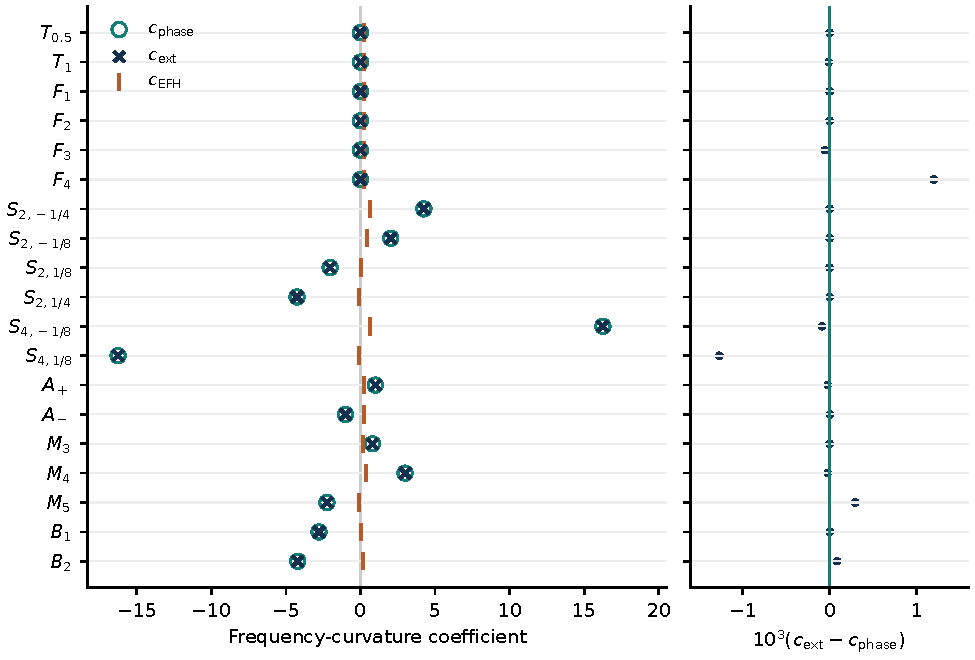
\includegraphics[width=\linewidth]{exhibits/curvature-comparison.pdf}
\caption{Smooth-profile curvature estimates. Left: the stored extrapolation
$\cext$ (crosses), the phase-integral value $\cphase$ (circles), and the
effective-horizon coefficient $\cefh$ (ticks). Right: the difference
$10^3(\cext-\cphase)$; no statistical error bars are assigned. All use
$\kappa=1$. The $A_-$ result is shown as a scattering comparison, but
lies outside the nonpositive-flow restriction of the effective-horizon
treatment. Overlap of crosses and circles on the left is resolved by
the residual panel.}
\label{fig:profiles}
\end{figure}
\begin{center}
\small
\begin{tabular}{@{}lrrrr@{}}
\toprule
Profile & $\Lambda_{\max}$ & $\cext$ & $\cphase$ & $\cefh$ \\
\midrule
$T_{0.5}$ & $80$ & $+0.000000$ & $+0.000000$ & $+0.250000$ \\
$T_1$ & $80$ & $-0.000009$ & $+0.000000$ & $+0.250000$ \\
$F_4$ & $80$ & $+0.001198$ & $+0.000000$ & $+0.250000$ \\
$S_{2,1/8}$ & $80$ & $-2.031250$ & $-2.031250$ & $+0.062500$ \\
$S_{4,1/8}$ & $80$ & $-16.251268$ & $-16.250000$ & $-0.125000$ \\
$A_+$ & $80$ & $+0.999977$ & $+1.000000$ & $+0.250000$ \\
$B_1$ & $320$ & $-2.778217$ & $-2.778220$ & $+0.040000$ \\
$B_2$ & $320$ & $-4.203465$ & $-4.203551$ & $+0.191500$ \\
\bottomrule
\end{tabular}

\end{center}
\noindent
The table gives selected values; displayed decimal places transcribe the
stored estimates and do not represent uncertainty bounds. The symmetric
profiles approach a curvature near zero rather than $1/4$. For the
shifted and mixed profiles, both signs and the scale of the measured
curvature follow Eq.~\eqref{eq:cphase}. The largest residuals in the
figure occur at $S_{4,1/8}$ and $F_4$, whose extrapolated discrepancies
are approximately $-0.001268$ and $+0.001198$. Thus uniform agreement
at the $10^{-4}$ level would overstate the whole-profile evidence.

\clearpage
\section{Cutoff dependence and the low-frequency offset}
\label{sec:convergence}
The four profiles extended to $\Lambda=320$ give the cutoff dependence in
Fig.~\ref{fig:convergence}. The curves use the stored finite-cutoff
coefficients, rather than an additional fit. Their approach to the
phase-integral values supports the interpretation of $c$ as the leading
curvature coefficient for these examples.
\begin{figure}[ht]
\centering
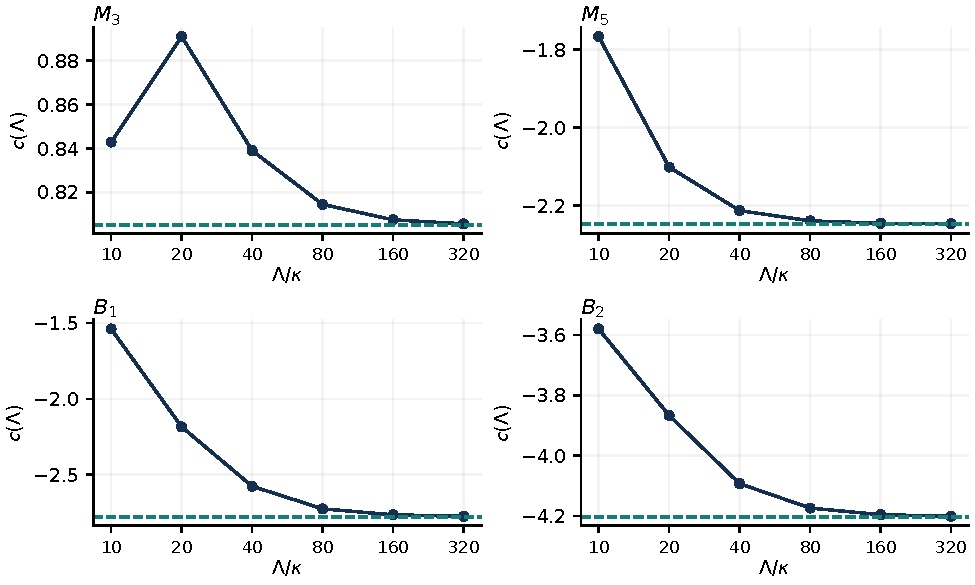
\includegraphics[width=\linewidth]{exhibits/curvature-convergence.pdf}
\caption{Cutoff dependence for two mixed and two held-out profiles. Points
are the quartic-frequency-fit coefficients $c(\Lambda)$ from
Eq.~\eqref{eq:fit}; dashed lines are Eq.~\eqref{eq:cphase}.
The logarithmic horizontal scale displays the six sampled cutoffs.
The curves join stored measurements only. Mesh refinement was recorded
at selected frequencies through $\Lambda=160$; the last points have no
such refinement check.}
\label{fig:convergence}
\end{figure}

\paragraph{The low-frequency intercept from the frequency fits.}
In units $\kappa=1$, the local formula derived formally in
Section~\ref{sec:b0} is
\begin{equation}
 \boxed{\bcand=\frac{v''''(0)-4v''(0)v'''(0)+3[v''(0)]^3}{12}.}
 \label{eq:bguess}
\end{equation}
For the held-out profiles the intercepts $\bext$ of the stored frequency
fits, Eq.~\eqref{eq:fit}, are
\begin{center}
\begin{tabular}{@{}lrrr@{}}
\toprule
Profile & $b_0(320)$ & $\bext$ & $\bcand$ \\
\midrule
$B_1$ & $-0.819600$ & $-0.815073$ & $-0.815076$ \\
$B_2$ & $+3.414518$ & $+3.416860$ & $+3.416864$ \\
\bottomrule
\end{tabular}

\end{center}
The absolute extrapolated differences are $2.93\times10^{-6}$ and
$3.69\times10^{-6}$, respectively. This is five-decimal-scale
agreement, conditional on the extrapolation, rather than an established
five-decimal error bound. The finite-$320$ offsets differ from
Eq.~\eqref{eq:bguess} by about $0.00452$ and $0.00235$, so the extrapolation
is material to the agreement. The leading phase integral in
Section~\ref{sec:phase} produces no frequency-independent $\Lambda^{-2}$
temperature term; Section~\ref{sec:b0} obtains this term from a separate
zero-frequency calculation.

\clearpage
\section{A formal derivation of the low-frequency offset}
\label{sec:b0}
This section obtains Eq.~\eqref{eq:bguess} in two stages. Stage~1 reduces
the $\omega\to0$ limit of $T_{\rm ratio}$ to a zero-frequency problem without
approximation in $\Lambda$. Stage~2 evaluates that limit by an expansion
about the horizon turning point. In general units the result reads
\begin{equation}
 \frac{T(0)}{\HawkingT}-1=\frac{b_0\kappa^2}{\Lambda^2}+O(\Lambda^{-4}),
 \qquad
 b_0=\frac{1}{12}\left[\frac{v''''}{\kappa^4}-\frac{4v''v'''}{\kappa^5}
 +\frac{3(v'')^3}{\kappa^6}\right]=\frac{g'''(0)}{12\kappa},
 \label{eq:b0}
\end{equation}
with derivatives of $v$ at the horizon, $T(0)=\lim_{\omega\to0}T_{\rm ratio}$,
and $O(\Lambda^{-4})$ the next order of the formal expansion. Here
$u=1+v$ and $g(u)=v'(x(u))$, with $x(u)$ the local inverse near the horizon,
so that $g(0)=\kappa$. If $g$ is regarded as a function of $v$ itself, the
evaluation point is $v=-1$. Equivalently, the relative offset is
$\kappa g'''(0)/(12\Lambda^2)$.

\subsection{Hypotheses, order of limits and assumptions}
\label{sec:hyp}
The flow $v(x)$ is real, smooth, independent of $\Lambda$ and monotone near
the horizon. It tends to constants $v_-<-1$ as $x\to-\infty$ and
$-1<v_+<1$ as $x\to+\infty$, with derivatives decaying at least
exponentially. The function $1-v^2$ vanishes only at the simple zero $x=0$;
in particular there is no second turning point, such as $v=+1$. The
scattering problem is nondegenerate, and the quantities $\mathcal{N}$ and $\mathcal{M}$
defined below satisfy $\mathcal{N}\neq0$ and $\mathcal{N}\mathcal{M}>0$. The limit $\omega\to0$ is taken
first at fixed $\Lambda$; the expansion in $1/\Lambda$ follows. No uniform
interchange of the two limits is claimed. The calculation further uses:
\begin{enumerate}
\item[(A1)] \emph{Low-frequency regularity and matching.} The outgoing-$u$
solution, suitably normalized, has an expansion $f_0+\omega f_1+O(\omega^2)$
on bounded intervals, and the boundary-condition determinant has no
exceptional zero at $\omega=0$. There is an overlap region outside the
flow transition but with $\omega|x|\ll1$, in which this expansion is
matched to the exterior soft waves and to the interior stiff waves.
\item[(A2)] \emph{Oscillatory tails.} Integrals over the interior stiff
oscillations are defined by Abel continuation (multiplication by
$e^{\epsilon x}$ and $\epsilon\downarrow0$), and this reproduces the
finite-frequency boundary conditions. In particular, setting $\omega=0$
before matching leaves no soft constant or slope absent at finite
$\omega$, so that the integration constants $K_0$ and $K$ below vanish.
\item[(A3)] \emph{Local evaluation.} To the order retained, the global
integrals $\mathcal{N}$, $\mathcal{M}$ and the Wronskian $W_c$ are given by termwise
integration of the local turning-point expansion; contributions from
regions away from the turning point are negligible to all orders kept.
This includes the travelling-wave normalization: the formal second solution
obtained by replacing $\Ai$ with $\Bi$ must combine with the first into the
single incoming stiff component that defines $W_c$, to the order retained.
\end{enumerate}
A1 and A2 are supported by the stage-wise numerical agreement below, and
for constant interior velocity A2 reproduces exactly the primitives
obtained from the finite-frequency stiff waves. None of A1--A3 is proved
here. A proof would require a controlled global matching, for example a
uniform Airy approximation near the turning point connected to WKB
solutions away from it, with explicit remainder bounds.

\subsection{Stage 1: reduction to a zero-frequency problem}
\label{sec:stage1}
Let $\phi^{\rm out}_u$ be the stationary solution containing, on the right,
only the outgoing $u$ wave, an incoming co-propagating wave and the decaying
evanescent solution, and on the left only the two incoming stiff waves.
Two left-hand outgoing soft channels and the growing right-hand solution are
excluded, which leaves one solution up to normalization. By
pseudo-unitarity, the magnitudes of its incoming coefficients are those of
the outgoing-$u$ row of $S$. Write $\phi^{\rm out}_u=E\,(f_0+\omega
f_1+\cdots)$ under A1 and $L_0f=\Lambda^{-2}f''''-[(1-v^2)f']'$. Then
Eq.~\eqref{eq:ode} gives
\begin{equation}
 L_0f_0=0,\qquad L_0f_1=i\,[(vf_0)'+vf_0'].
\end{equation}
Integrating the first equation once, with vanishing constant $K_0$ (A2),
gives $f_0'=\psi/\mathcal{N}$, where $\psi$ is a real solution of
\begin{equation}
 \psi''=\Lambda^2(1-v^2)\,\psi
 \label{eq:psi}
\end{equation}
that decays as $x\to+\infty$. It is unique up to normalization, and all
results below are invariant under rescaling of $\psi$. On the left,
$\psi\simeq b\,e^{ikx}+b^*e^{-ikx}$ with $k=\Lambda\sqrt{v_-^2-1}$. With
$\mathcal{N}=\int\psi\,\dd x$ (Abel continuation on the left, A2) and
$f_0=\mathcal{N}^{-1}\int_{-\infty}^x\psi$, $f_0$ tends to $1$ on the right and is a
purely stiff oscillation on the left.

The once-integrated first-order equation is
$\Lambda^{-2}f_1'''-(1-v^2)f_1'=i[vf_0+\int_{-\infty}^x vf_0']+K$ with
$K=0$ (A2). On the right, $f_1'\to-i(v_++I_v)/(1-v_+^2)$, where
\begin{equation}
 I_v=\int vf_0'\,\dd x=-1-\delta,\qquad
 \delta=-\frac{1}{\mathcal{N}}\int(1+v)\,\psi\,\dd x .
\end{equation}
The exterior soft waves have $k_u=\omega/(1+v_+)+\cdots$ and
$k_v=-\omega/(1-v_+)+\cdots$. Both have $|\Omega_cv_g|=\omega+o(\omega)$,
so their leading flux normalizations agree, and the exterior solution is
$\omega^{-1/2}[e^{ik_ux}+c_ve^{ik_vx}]$. Matching constant and slope terms in
the overlap region of A1 gives
\begin{equation}
 E=\omega^{-1/2}(1+c_v),\qquad
 c_v=\frac{1+I_v}{1-I_v}=-\frac{\delta}{2+\delta}.
\end{equation}

On the left the stiff part of $f_0$ has amplitude $a=b/(ik\mathcal{N})$, and
$\Omega_cv_g=k(v_-^2-1)$ at $\omega=0$. Hence
\begin{equation}
 |\beta|^2\simeq|E|^2F,\qquad
 F=|a|^2\Lambda(v_-^2-1)^{3/2}=\frac{|W_c|}{2\Lambda^2\mathcal{N}^2},
\end{equation}
where $W[f,h]=fh'-f'h$ and $W_c=W[\psi_c,\psi_c^*]$. Here $\psi_c$ is the
solution of Eq.~\eqref{eq:psi} whose left asymptotic form is the
positive-wave-number wave $b\,e^{ikx}$, so that $\psi=\psi_c+\psi_c^*$ and
$W_c=-2ik|b|^2$, independent of $x$. Only $|W_c|$ enters below.
Since $|\beta|^2\sim1/\omega$,
$\log(|\alpha|^2/|\beta|^2)=\log[1+(1-G)/|\beta|^2]=\omega(1-G_0)/C_\beta+o(\omega)$,
with $C_\beta=\lim\omega|\beta|^2=|1+c_v|^2F=4F/(2+\delta)^2$ and
$G_0=\lim G=c_v^2=\delta^2/(2+\delta)^2$. Therefore
\begin{equation}
 \boxed{T(0)=\frac{C_\beta}{1-G_0}=\frac{F}{1+\delta}
 =\frac{|W_c|}{2\Lambda^2\mathcal{N}\mathcal{M}},\qquad \mathcal{M}=\int(-v)\,\psi\,\dd x=\mathcal{N}(1+\delta).}
 \label{eq:T0}
\end{equation}
Stage~1 makes no approximation in $\Lambda$; it holds under the hypotheses
of Section~\ref{sec:hyp}, A1 and A2. The order-$\Lambda^{-2}$ dependence on
$\delta$ enters through $C_\beta=|1+c_v|^2F$; the factor $1/(1-G_0)$ changes
$T(0)$ only at order $\Lambda^{-4}$, because $G_0=O(\Lambda^{-4})$. With
$T_n=\omega/\log(1+1/|\beta|^2)$ one has $T_n(0)=C_\beta=T(0)(1-G_0)$, so
the two definitions share $b_0$. The first-order calculation determines
$T(0)$ only. It does not show that $T_{\rm ratio}(\omega)-T(0)$ is of order
$\omega^2$; the even-power fits of Section~\ref{sec:computed} assume that
form.

As a normalization check at leading order, replace the potential by its
linearization $1-v^2\simeq2x$ ($\kappa=1$). Then $\psi=\Ai(sx)$ with
$s=(2\Lambda^2)^{1/3}$, and $|W_c|=s/(2\pi)$, $\mathcal{N}=\mathcal{M}=1/s$ give
$T(0)=1/(2\pi)=\HawkingT$. This checks the linearized problem only. For an
exactly linear velocity, $1-v^2=2x-x^2$, and $\Ai(sx)$ is not a solution.

\subsection{Stage 2: expansion about the turning point}
\label{sec:stage2}
Write $u=1+v=x+a_2x^2+a_3x^3+\cdots$ with $a_n=v^{(n)}(0)/n!$ and
$\kappa=1$. Put $x=\varepsilon y$ with $2\Lambda^2\varepsilon^3=1$, so that
$\Lambda^{-2}=2\varepsilon^3$. Equation~\eqref{eq:psi} becomes
$\psi_{yy}=V(y)\psi$ with
\begin{equation}
 V=\frac{2u-u^2}{2\varepsilon}=y+\varepsilon c_1y^2+\varepsilon^2c_2y^3
 +\varepsilon^3c_3y^4+\cdots,\quad
 c_1=a_2-\tfrac12,\ c_2=a_3-a_2,\ c_3=a_4-a_3-\tfrac12a_2^2 .
\end{equation}
With $\mathcal{N}=\varepsilon I_N$, $\mathcal{M}=\varepsilon I_M$ and
$|W_c|=W_y[\psi_{\Ai},\psi_{\Bi}]/(2\varepsilon)$, Eq.~\eqref{eq:T0} becomes
\begin{equation}
 \frac{T(0)}{\HawkingT}=\frac{\pi\,W_y[\psi_{\Ai},\psi_{\Bi}]}{I_N\,I_M},\qquad
 I_N=\int\psi\,\dd y,\quad I_M=\int(1-u)\,\psi\,\dd y .
 \label{eq:Ty}
\end{equation}
Here $W_y[\Ai,\Bi]=1/\pi$. For $y\to-\infty$, $\Ai\sim A\sin\theta$ and
$\Bi\sim A\cos\theta$ with $\theta=\tfrac23(-y)^{3/2}+\tfrac\pi4$
decreasing in $y$, so the positive-wave-number component is
$\psi_c=\tfrac12(\psi_{\Ai}+i\psi_{\Bi})$. This identification, which
fixes the Wronskian factor, is the travelling-wave normalization contained
in A3; the opposite choice of sign changes only the sign of $W_c$.

Each order is sought in the form $\psi_n=P_n\Ai+Q_n\Ai'$ with polynomials
$P_n,Q_n$. The identity
$(\partial_y^2-y)(P\Ai+Q\Ai')=(P''+2yQ'+Q)\Ai+(2P'+Q'')\Ai'$ turns each
order into a triangular recursion for the polynomial coefficients. The only
freedom is the normalization of $\psi$, which cancels in
Eq.~\eqref{eq:Ty}. Since $\Bi$ cannot be written in this form, the decaying
condition on the subsonic side is built in. Replacing $\Ai$ by $\Bi$ with
the same $P,Q$ gives the formal second solution, and
$\pi W_y=P^2+PQ'-QP'-yQ^2$, which is independent of $y$ at each order.
The integrals use the Abel-regularized Airy moments
$\int y^{3j}\Ai\,\dd y=(3j)!/(3^jj!)$, with the other moments vanishing,
and $\int y^n\Ai'\,\dd y=-n\int y^{n-1}\Ai\,\dd y$. The first correction is
$\psi_1=\tfrac{c_1}{5}(y^2\Ai'-y\Ai)$.

With $P_0=1$ and no constant term added at higher orders, the
$\varepsilon^1$ and $\varepsilon^2$ terms of $\pi W_y$, $I_N$ and $I_M$
vanish, and the $\varepsilon^3$ coefficients are
\begin{equation}
 [I_N]_3=-\tfrac{422}{225}c_1^3+\tfrac{166}{45}c_1c_2-\tfrac{16}{9}c_3,\qquad
 [\pi W_y]_3=\tfrac{56}{225}c_1^3-\tfrac{28}{45}c_1c_2+\tfrac49c_3,\qquad
 [\delta]_3=-\tfrac12-a_2,
\end{equation}
with $[I_M]_3=[I_N]_3+[\delta]_3$. Combining them,
\begin{equation}
 \Big[\frac{T(0)}{\HawkingT}\Big]_3=4c_1^3-8c_1c_2+4c_3+\tfrac12+a_2
 =4a_4-8a_2a_3+4a_2^3 .
\end{equation}
Since $\varepsilon^3=\Lambda^{-2}/2$, this is
$b_0=2a_4-4a_2a_3+2a_2^3$, i.e.\ Eq.~\eqref{eq:bguess}; restoring $\kappa$
gives Eq.~\eqref{eq:b0}. The expansion through $\varepsilon^6$, including
$b_0$ and $b_1$ below, was reproduced by a second, independently written
exact calculation that starts from the differential equation. The same
calculation gives $\delta=-(1+v'')/(4\Lambda^2)+O(\Lambda^{-4})$, hence
$G_0\simeq(1+v'')^2/(64\Lambda^4)$ ($\kappa=1$); in general units,
$\delta=-(\kappa^2+v'')/(4\Lambda^2)+\cdots$ and
$G_0\simeq(\kappa^2+v'')^2/(64\Lambda^4)$. The corrections to $F$ and to $\delta$
share the term $-(1+v'')/4$, which cancels in $F/(1+\delta)$; neither
quantity alone gives $b_0$.

Carried to $\varepsilon^6$ (derivatives through $v^{(7)}$), the expansion
of $T(0)/\HawkingT-1$ has nonzero terms only at $\varepsilon^3$ and
$\varepsilon^6$: through this order it proceeds in powers of
$\Lambda^{-2}$. The $\varepsilon^6$ term defines the next coefficient $b_1$
in $T(0)/\HawkingT-1=b_0/\Lambda^2+b_1/\Lambda^4+\cdots$ ($\kappa=1$), a
polynomial of 28 terms in the Taylor coefficients, or of 18 terms in the
coefficients of $g$, Eq.~\eqref{eq:b1} in Appendix~\ref{app:b1}. Because
$T_n(0)=T(0)(1-G_0)$, $b_1$ refers to $T_{\rm ratio}$, while $b_0$ is
common to both definitions.

In terms of $g$, write $u'=g(u)=\kappa+g_1u+g_2u^2+g_3u^3+\cdots$. At
$\kappa=1$, $v''=g_1$, $v'''=g_1^2+2g_2$ and $v''''=g_1^3+8g_1g_2+6g_3$,
so $b_0=g_3/2=g'''(0)/12$. For Riccati flows $u'=\kappa+\beta u+\gamma u^2$,
which include $T_D$ and all $S_{q,t}$, $g'''=0$ and $b_0=0$. This does not
make $T(0)$ equal to $\HawkingT$ at finite $\Lambda$, since $b_1\neq0$ in
general.

\subsection{Numerical checks of each stage}
\label{sec:checks}
For seven profiles, Eq.~\eqref{eq:psi} is integrated from the subsonic side
inward, with the asymptotic tails added in closed form, to give $\mathcal{N}$, $\mathcal{M}$,
$W_c$, $F$ and $\delta$. Independently, the boundary-value method gives
$\omega\to0$ limits of $T_{\rm ratio}$, $C_\beta$ and $G$ as described in
Section~\ref{sec:computed}. Table~\ref{tab:b0} and Fig.~\ref{fig:b0}
summarize the comparison.
\begin{table}[ht]
\centering
\small
\begin{tabular}{@{}lrrrrrr@{}}
\toprule
Profile & $b_0$ (Eq.~\eqref{eq:b0}) & $b_0$ from scattering & difference & $\max|\Delta T(0)|/\HawkingT$ & $b_1$ (local) & $b_1$ (fit) \\
\midrule
$T_{0.5}$ & $+0.000000$ & $+0.000000$ & $-6.8\times10^{-8}$ & $1.1\times10^{-11}$ & $+0.25000$ & $+0.24996$ \\
$S_{2,1/4}$ & $+0.000000$ & $-0.000001$ & $-1.1\times10^{-6}$ & $1.3\times10^{-10}$ & $+0.81250$ & $+0.81245$ \\
$A_+$ & $-1.000000$ & $-1.000000$ & $+1.6\times10^{-7}$ & $3.4\times10^{-11}$ & $+0.18750$ & $+0.18723$ \\
$M_4$ & $-1.620000$ & $-1.620090$ & $-9.0\times10^{-5}$ & $1.6\times10^{-11}$ & $-53.41988$ & $-53.43998$ \\
$B_2$ & $+3.416864$ & $+3.417799$ & $+9.3\times10^{-4}$ & $2.0\times10^{-11}$ & $-239.75501$ & $-240.02570$ \\
\midrule
$B_3$ & $-0.607006$ & $-0.607006$ & $+1.0\times10^{-7}$ & $1.2\times10^{-11}$ & $-2.24793$ & $-2.24798$ \\
$B_4$ & $+1.133602$ & $+1.133602$ & $-1.4\times10^{-8}$ & $5.8\times10^{-12}$ & $+0.57353$ & $+0.57350$ \\
\bottomrule
\end{tabular}

\caption{Low-frequency offset, $\kappa=1$. Second column: Eq.~\eqref{eq:b0}
from the Taylor coefficients. Third: extrapolation of the (extrapolated) $\omega\to0$ scattering limits
$\Lambda^2[T(0)/\HawkingT-1]$ at $\Lambda=20,40,80$ in $\Lambda^{-2}$ and
$\Lambda^{-4}$; fourth: third minus second. Fifth: largest difference
between the scattering limit and Eq.~\eqref{eq:T0} over $\Lambda=10$--$80$.
Last two columns: $b_1$ from the local expansion and from a fit of the
zero-frequency formula at $\Lambda=28$--$80$ (relative tolerance
$10^{-13}$). $B_3$ and $B_4$, below the rule, are the prediction-first
families.}
\label{tab:b0}
\end{table}

\emph{Stage 1.} Over all 28 cases ($\Lambda=10,20,40,80$) the extrapolated
scattering limit, a four-point extrapolation from $\omega\geq0.0025$, and
Eq.~\eqref{eq:T0} differ by at most $1.3\times10^{-10}$ in
$T(0)/\HawkingT$. Refitting the same stored solves on the three smallest or
the three largest frequencies, quadratically in $\omega^2$, changes the
extrapolated value by at most $1.4\times10^{-10}$, while the value at the
smallest frequency alone differs from Eq.~\eqref{eq:T0} by up to
$2.7\times10^{-7}$. The pseudo-unitarity residual of the solves, below
$1.9\times10^{-9}$, is a conservation diagnostic, not a bound on the
temperature or extrapolation error. The limits $G_0$ agree with
$\delta^2/(2+\delta)^2$ within a relative $8.4\times10^{-7}$. The agreement
of $C_\beta$ adds no independent content, since $T(0)=C_\beta/(1-G_0)$
identically.

\emph{Stage 2.} The difference between $\Lambda^2\delta$ and the local value
$-(1+v'')/4$ decreases, from $\Lambda=40$ on, by a factor of three to four
per doubling of $\Lambda$, to at most $4.8\times10^{-3}$ at $\Lambda=80$ and
$3.0\times10^{-4}$ at $\Lambda=320$ (five profiles). The extrapolated $b_0$ agrees with Eq.~\eqref{eq:b0} within
$1.2\times10^{-6}$ except for $M_4$ and $B_2$. For those two profiles,
large $\Lambda^{-6}$ terms limit the three-point extrapolation from
$\Lambda\leq80$; the frequency-fit intercept of Section~\ref{sec:convergence},
which uses cutoffs up to $320$, is $3.416860$ for $B_2$. Subtracting
$b_1/\Lambda^2$ from the zero-frequency value of $\Lambda^2[T(0)/\HawkingT-1]$
at $\Lambda=320$ reproduces $b_0$ within $6.3\times10^{-6}$ ($M_4$) and
$8.6\times10^{-6}$ ($B_2$). The fitted $b_1$ agrees with the local
expansion within $0.15\%$ for all seven profiles.
\begin{figure}[ht]
\centering
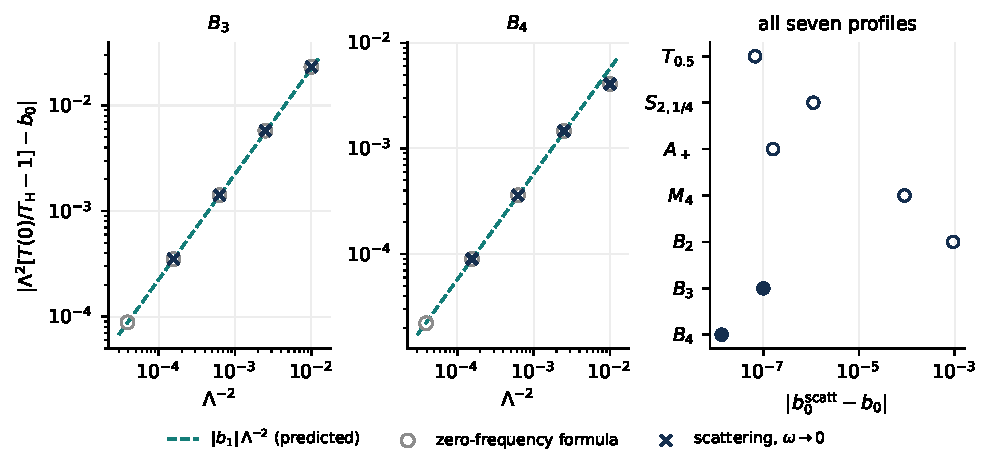
\includegraphics[width=.9\linewidth]{exhibits/b0-comparison.pdf}
\caption{Low-frequency offset, $\kappa=1$. Left and centre: for the
prediction-first families, the deviation of $\Lambda^2[T(0)/\HawkingT-1]$
from the predicted $b_0$, from the zero-frequency formula
Eq.~\eqref{eq:T0} (circles, $\Lambda=10$--$160$) and from the scattering
limits (crosses, $\Lambda=10$--$80$). The dashed line is the predicted next
term $|b_1|\Lambda^{-2}$, with no fitted parameter. Right: absolute
difference between the extrapolated and the predicted $b_0$ for all seven
profiles of Table~\ref{tab:b0}; filled markers are the prediction-first
families.}
\label{fig:b0}
\end{figure}

\subsection{Prediction-first test}
\label{sec:blind}
For $B_3$ and $B_4$, Eq.~\eqref{eq:newprofiles}, the predictions of $b_0$,
$b_1$ and $\delta$ were recorded before any zero-frequency or scattering
calculation for these families. They used only the local formulas and
Taylor coefficients from complex Cauchy integrals (two radii agree within
$3.1\times10^{-10}$ for $B_3$ and $8.4\times10^{-8}$ for $B_4$). The success criteria were fixed at the same
time: (1) $b_0$ extrapolated from the extrapolated scattering limits at
$\Lambda=20,40,80$, with basis $b_0+e_1\Lambda^{-2}+e_2\Lambda^{-4}$,
agrees with the prediction within $10^{-3}\max(1,|b_0|)$;
(2) Eq.~\eqref{eq:T0} agrees with the extrapolated scattering limit within $10^{-9}$ in $T(0)/\HawkingT$ at every computed $\Lambda$;
(3) as a secondary test, $b_1$ from the zero-frequency formula at
$\Lambda=20$--$160$ agrees within $10\%$. All three are met for both
families. The differences in (1) are $+1.0\times10^{-7}$ ($B_3$,
predicted $b_0=-0.6070063$) and $-1.4\times10^{-8}$ ($B_4$,
$b_0=+1.1336018$). For (2) the largest differences are
$1.2\times10^{-11}$ and $5.8\times10^{-12}$. For (3) the fits give
$-2.2601$ and $0.5685$ against the predicted $-2.2479$ and $0.5735$;
the refined fits of Table~\ref{tab:b0} give $-2.24798$ and $0.57350$.
With the alternative three-frequency windows of Section~\ref{sec:checks},
the differences in (1) become $+1.0\times10^{-7}$ and $+1.1\times10^{-7}$
($B_3$), and $-1.3\times10^{-8}$ and $-1.3\times10^{-9}$ ($B_4$).

Fixed before any zero-frequency or scattering result for these profiles
were the profiles, the predictions, the three criteria, the cutoffs and
basis of criterion (1), the frequencies and $\omega\to0$ extrapolation
bases of Section~\ref{sec:computed}, the boundary-value discretization and
the integrator tolerance. The cutoff list actually run,
$\Lambda=10,20,40,80,160$, is consistent with the criteria but was set at
run time. Two choices were made later, with the results available. For
(3), the basis is a least-squares fit of
$\Lambda^4[T(0)/\HawkingT-1]-\Lambda^2b_0$ by
$b_1+e\Lambda^{-2}+e'\Lambda^{-4}$ at $\Lambda=20,40,80,160$, with $b_0$
fixed at its predicted value. The refined fits of Table~\ref{tab:b0} use the
same basis at $\Lambda=28,40,56,80$, from a later run at
$\Lambda=10,14,20,28,40,56,80$ with tolerance $10^{-13}$. A first parameter
choice for $B_3$ was rejected before any zero-frequency or scattering
calculation, because its right-hand asymptotic velocity was positive. These
are prediction-first tests by the same investigators, not blinded
experiments. They differ from the held-out profiles $B_1$, $B_2$ of
Section~\ref{sec:computed}, which were held out for the curvature
comparison; the $b_0$ comparisons for $B_1$, $B_2$ in Section~\ref{sec:convergence}
and for $B_2$ in Table~\ref{tab:b0} are not part of this protocol. This test does not
replace a proof of A1--A3. The independent numerical check of
Section~\ref{sec:computed} adds two further new profiles, $N_1$ and $N_2$.

\subsection{Relation to previous work}
The procedure of Stage~1 is that of Coutant and Weinfurtner
\cite{CWKdV,CWBdG}. In their Korteweg--de~Vries and Bogoliubov--de~Gennes
analyses the zero-frequency problem is reduced to a second-order equation,
the solution that does not grow on the subsonic side is selected, and
amplitudes are read from spatial integrals and asymptotic coefficients. In
the Bogoliubov--de~Gennes case the matching is carried to first order in
the frequency, which separates the exterior counter- and co-propagating
channels, and oscillatory integrals are given a regularized meaning. We transfer this procedure to Eq.~\eqref{eq:ode};
the integral weights and the form of Eq.~\eqref{eq:T0} follow from the
present operator, not from substitution into their coefficients. The Airy
expansion about a turning point and the use of the inverse flow, as in
Leonhardt and Robertson's Appendix~B \cite{LR}, are standard tools.
Himemoto and Tanaka's Eqs.~(5.2)--(5.5) \cite{HT} already allow
$\Lambda^{-2}$ corrections involving $v''''$, $v''v'''$ and $(v'')^3$,
with coefficient functions left unevaluated and under different dispersion
and connection conditions. What this section adds is the explicit
$\Lambda^{-2}$ coefficient, Eq.~\eqref{eq:b0}, for smooth single-horizon
flows in the present model that satisfy the hypotheses of
Section~\ref{sec:hyp}, as a formal result conditional on A1--A3. We have
not found this coefficient in the sources examined, but cannot exclude an
earlier statement elsewhere.

\clearpage
\section{Precision, interpretation, and remaining analytical questions}
\label{sec:discussion}
\paragraph{What the two-method comparison establishes.}
The symmetric-tanh comparison contains 93 numerical table entries
representing 64 distinct parameter points; repeated points occur in
tables printed at different precisions. Of these entries, 79 pass every
printed-field comparison using half the last printed unit, multiplied
by $1.0001$, plus $10^{-12}$. The other 14 fail this criterion for a
temperature shift; their largest excess over the printed half-unit is
below $9.4\times10^{-11}$ in $T/\HawkingT-1$. All three above-cutoff entries
agree. Absolute differences in coarsely printed $T/\HawkingT$ are below
$5.0\times10^{-7}$; the digits of those tables limit the comparison.
This is numerical compatibility at the recorded precision, with the
small discrepancies stated, rather than exact agreement of every
printed digit.

For this comparison set, the boundary-value method's maximum
$\|S^\dagger\eta S-\eta\|_{\max}$ is below $8.8\times10^{-12}$,
and its recorded refinement changes $T/\HawkingT$ by less than
$6.0\times10^{-13}$. For the full smooth-profile scans the corresponding
maximum norm residual is below $1.24\times10^{-9}$, the maximum recorded
current variation below $1.84\times10^{-9}$, and 64 selected refined-mesh
checks change the row temperature by less than $1.22\times10^{-10}$.
The current variation is normalized by the larger of one and the maximum
absolute current in a solution. These diagnostics test conservation and
discretization at sampled points; they are not bounds on coefficient
extrapolation. Multiplication by $\Lambda^2$ and extraction of a weak
frequency curvature amplify small temperature errors.

\paragraph{Temperature definitions.}
The calculation also records the column ratio
$T_{\rm col}=\omega/\log(|S_{u,+}|^2/|S_{P,+}|^2)$ and the
occupation-number temperature $T_n=\omega/\log(1+1/|\beta|^2)$. In
$T_{\rm col}$, $+$ labels the positive-norm incoming high-wave-number
channel and $P$ the negative-norm outgoing long-wavelength channel on the
left.
With $N=|\beta|^2$, our principal definition is instead
\begin{equation}
 T_{\rm ratio}=\frac{\omega}{\log[1+(1-G)/N]}.
\end{equation}
Channel coupling must therefore be controlled at the order being compared;
the three temperatures are not interchangeable by definition. Separating
an offset and a curvature, as in Macher--Parentani Eqs.~(42)--(45)
\cite{MP}, also prevents an intercept from being misidentified as a
frequency correction.

\paragraph{How to interpret the effective-horizon comparison.}
The finite-scattering coefficients differ from a direct use of
Eq.~\eqref{eq:cefh} on these backgrounds. Three analytical questions remain.
First, the terms omitted in the approximant and adiabatic constructions
\cite{DPLS25,DPLS} need an error estimate at the order $\Lambda^{-2}$, rather than only at
the leading thermal order. Second, one must compare an effective-horizon
peeling slope with the logarithmic coefficient relevant to the normalized
full-scattering ratio. Third, fixed-$\omega/\kappa$ weak dispersion and
the subsequent $\omega\to0$ limit need compatible, preferably uniform,
control. These are possible explanations to investigate; none is
identified as the cause by the present data. No claim that the
effective-horizon analysis is erroneous follows from this comparison.

\paragraph{Conclusion.}
Full-scattering measurements over the specified smooth profiles support
the curvature obtained from a known phase-integral formula. Two distinct
numerical methods check the symmetric reference cases, while the wider
profile set tests the derivative dependence with the boundary-value
method. The low-frequency offset is obtained by a formal zero-frequency
calculation, supported by stage-wise numerical checks, by two
prediction-first families and by an independent computation on four
profiles. The main analytical task that remains is to
prove assumptions A1--A3 with a controlled remainder, for the stated class
of flows and order of limits. Carrying the same matching to second order in
the frequency might also give $c$ within the full-scattering framework; this
has not been attempted.
More generally, broadened-horizon analyses \cite{FP,CP} motivate testing
which aspects of a correction are local and which depend on the
surrounding flow.

\paragraph{AI use.}
AI systems assisted with numerical implementation and analysis,
the low-frequency asymptotic calculation and its exact algebra, an
independent check of that calculation, literature comparison, algebraic exposition, English drafting, figures
and consistency checks. The human author retains responsibility for
the content and its stated scope; AI systems are not authors. The
article has not undergone human expert review.

\appendix
\section{The next coefficient \texorpdfstring{$b_1$}{b1}}
\label{app:b1}
With $\kappa=1$ and $g(u)=1+\sum_{n\geq1}g_nu^n$, the $\varepsilon^6$ term
of the formal expansion gives the coefficient of $\Lambda^{-4}$ in
$T(0)/\HawkingT-1$ as
\begin{align}
 b_1={}&\tfrac{1}{2}g_1g_2g_3+\tfrac{7}{2}g_1g_5+\tfrac{3}{4}g_1^2g_4+2g_2g_4+g_3^2+3g_6\nonumber\\
 &+g_1g_4+\tfrac{1}{8}g_1^2g_3+\tfrac{1}{2}g_2g_3+g_5+\tfrac{1}{8}g_1g_3-\tfrac{1}{16}g_1^2g_2\nonumber\\
 &+\tfrac{1}{4}g_4-\tfrac{1}{8}g_1g_2-\tfrac{1}{32}g_1^3-\tfrac{1}{16}g_1^2-\tfrac{1}{16}g_2-\tfrac{1}{32}g_1.
 \label{eq:b1}
\end{align}

For $T_{0.5}$, $g=1-4u^2$ and $b_1=1/4$. With $g_n$ obtained from the Taylor
coefficients of $B_3$ and $B_4$, Eq.~\eqref{eq:b1} reproduces the predicted
values of Table~\ref{tab:b0}. Like $b_0$, Eq.~\eqref{eq:b1} is a formal
coefficient, conditional on A1--A3.

\clearpage
\begin{thebibliography}{13}
\bibitem{CJ}
S. Corley and T. Jacobson,
``Hawking spectrum and high frequency dispersion,''
\emph{Phys. Rev. D} \textbf{54}, 1568 (1996),
\href{https://arxiv.org/abs/hep-th/9601073v1}{arXiv:hep-th/9601073v1}.

\bibitem{US}
W. G. Unruh and R. Sch\"utzhold,
``On the universality of the Hawking effect,''
\emph{Phys. Rev. D} \textbf{71}, 024028 (2005),
\href{https://arxiv.org/abs/gr-qc/0408009v2}{arXiv:gr-qc/0408009v2}.

\bibitem{MP}
J. Macher and R. Parentani,
``Black/White hole radiation from dispersive theories,''
\emph{Phys. Rev. D} \textbf{79}, 124008 (2009),
\href{https://arxiv.org/abs/0903.2224v3}{arXiv:0903.2224v3}.

\bibitem{CPF}
A. Coutant, R. Parentani and S. Finazzi,
``Black hole radiation with short distance dispersion, an analytical
S-matrix approach,'' \emph{Phys. Rev. D} \textbf{85}, 024021 (2012),
\href{https://arxiv.org/abs/1108.1821v3}{arXiv:1108.1821v3}.

\bibitem{LR}
U. Leonhardt and S. Robertson,
``Analytical theory of Hawking radiation in dispersive media,''
\emph{New J. Phys.} \textbf{14}, 053003 (2012),
\href{https://doi.org/10.1088/1367-2630/14/5/053003}{doi:10.1088/1367-2630/14/5/053003}.

\bibitem{HT}
Y. Himemoto and T. Tanaka,
``Generalization of the model of Hawking radiation with modified high
frequency dispersion relation,'' \emph{Phys. Rev. D} \textbf{61}, 064004 (2000),
\href{https://arxiv.org/abs/gr-qc/9904076v3}{arXiv:gr-qc/9904076v3}.

\bibitem{MRB}
A. Moreno-Ruiz and D. Bermudez,
``Hawking temperature in dispersive media: Analytical and numerical study,''
\href{https://arxiv.org/abs/1908.02368v1}{arXiv:1908.02368v1} (2019),
\href{https://doi.org/10.1016/j.aop.2020.168268}{doi:10.1016/j.aop.2020.168268}.

\bibitem{DPLS25}
F. Del Porro, S. Liberati and M. Schneider,
``Tunneling method for Hawking quanta in analogue gravity,''
\emph{C. R. Phys.} \textbf{25}, S2, 1--27 (2024; published online 24 Feb 2025),
\href{https://doi.org/10.5802/crphys.239}{doi:10.5802/crphys.239},
\href{https://arxiv.org/abs/2406.14603v2}{arXiv:2406.14603v2}.

\bibitem{DPLS}
F. Del Porro, S. Liberati and M. Schneider,
``Hawking radiation with dispersion: reconciling the Bogoliubov and
tunneling approaches,''
\href{https://arxiv.org/abs/2604.24861v1}{arXiv:2604.24861v1} (2026).

\bibitem{CWKdV}
A. Coutant and S. Weinfurtner,
``Low frequency analogue Hawking radiation: The Korteweg--de Vries model,''
\emph{Phys. Rev. D} \textbf{97}, 025005 (2018),
\href{https://arxiv.org/abs/1707.09651v2}{arXiv:1707.09651v2}.

\bibitem{CWBdG}
A. Coutant and S. Weinfurtner,
``Low frequency analogue Hawking radiation: The Bogoliubov--de Gennes model,''
\emph{Phys. Rev. D} \textbf{97}, 025006 (2018),
\href{https://arxiv.org/abs/1707.09664v2}{arXiv:1707.09664v2}.

\bibitem{FP}
S. Finazzi and R. Parentani,
``Spectral properties of acoustic black hole radiation: Broadening the
horizon,'' \emph{Phys. Rev. D} \textbf{83}, 084010 (2011),
\href{https://arxiv.org/abs/1012.1556v2}{arXiv:1012.1556v2}.

\bibitem{CP}
A. Coutant and R. Parentani,
``Hawking radiation with dispersion: The broadened horizon paradigm,''
\emph{Phys. Rev. D} \textbf{90}, 121501 (2014),
\href{https://arxiv.org/abs/1402.2514v2}{arXiv:1402.2514v2}.
\end{thebibliography}
\end{document}
